\documentclass{beamer}
%\documentclass[handout]{beamer}

\usetheme{Copenhagen}
\usecolortheme{seahorse}


% for handouts, use with
% \documentclass[handout]{beamer}
%\usepackage{pgfpages}
%\pgfpagesuselayout{4 on 1}[a4paper, border shrink=5mm]


% hide navigation butons at bottom
\setbeamertemplate{navigation symbols}{}

%hide navigation at top
\setbeamertemplate{headline}{}

\setbeamercovered{transparent}


\usepackage[ngerman]{babel}
\babelprovide[hyphenrules=ngerman-x-latest]{ngerman}

\usepackage{csquotes}
\usepackage[backend=biber]{biblatex}
\addbibresource{../Ausarbeitung/Proseminar.bib}

\usepackage{graphicx}
\usepackage{float}
\usepackage{caption}
\usepackage{standalone}
\usepackage{nicefrac}

\usepackage{tikz}
\usepackage[europeanresistors]{circuitikz}
\usetikzlibrary{decorations.markings}
\usetikzlibrary{arrows.meta}
\usetikzlibrary{calc}

\usepackage{pgfplots}
\pgfplotsset{compat=1.18}


\title{Übertragung von Signalen auf elektrischen Leitungen}
\author{Sven Schmidt}


%Display page with section title at the beginning of each section
\AtBeginSection[]{
    \begin{frame}
        \centering
        \vfill
        \huge \insertsectionhead
        \vfill
    \end{frame}
}


\begin{document}

% Title page with image at the top
\begin{frame}
    \centering
    % Insert and center the image at the top
    
\includegraphics[width=0.5\textwidth]{logo_fernuni_hagen.png}
    \vspace{0.5cm} % Adjust space between image and title as needed

    {\LARGE \textbf{\inserttitle}}\\[0.5cm]

    \textbf{Proseminar Mathematik in der Technik}\\
    \textbf{Modulnummer:} 61711\\
    Fakultät für Mathematik + Informatik\\[0.5cm]

    \begin{tabbing}
        \hspace{4cm} \= \kill
        \textbf{Name:} \> Sven Schmidt \\
        \textbf{Matrikelnummer:} \> 4125169 \\
        \textbf{Prüfer:} \> PD Dr.-Ing. Stefan Helfert \\
    \end{tabbing}

    \vfill

    {\large FernUniversität in Hagen}\\
    {\large Sommersemester 2025}
\end{frame}

\begin{frame}{Inhalt}
    \tableofcontents
\end{frame}

\section{Herleitung der Telegraphenleitung}


\begin{frame}{Modell des Zweidrahtleiters}

Wir betrachten ausschließlich Paralleldrahtleiter.

\begin{figure}[!htb]
    \begin{center}
        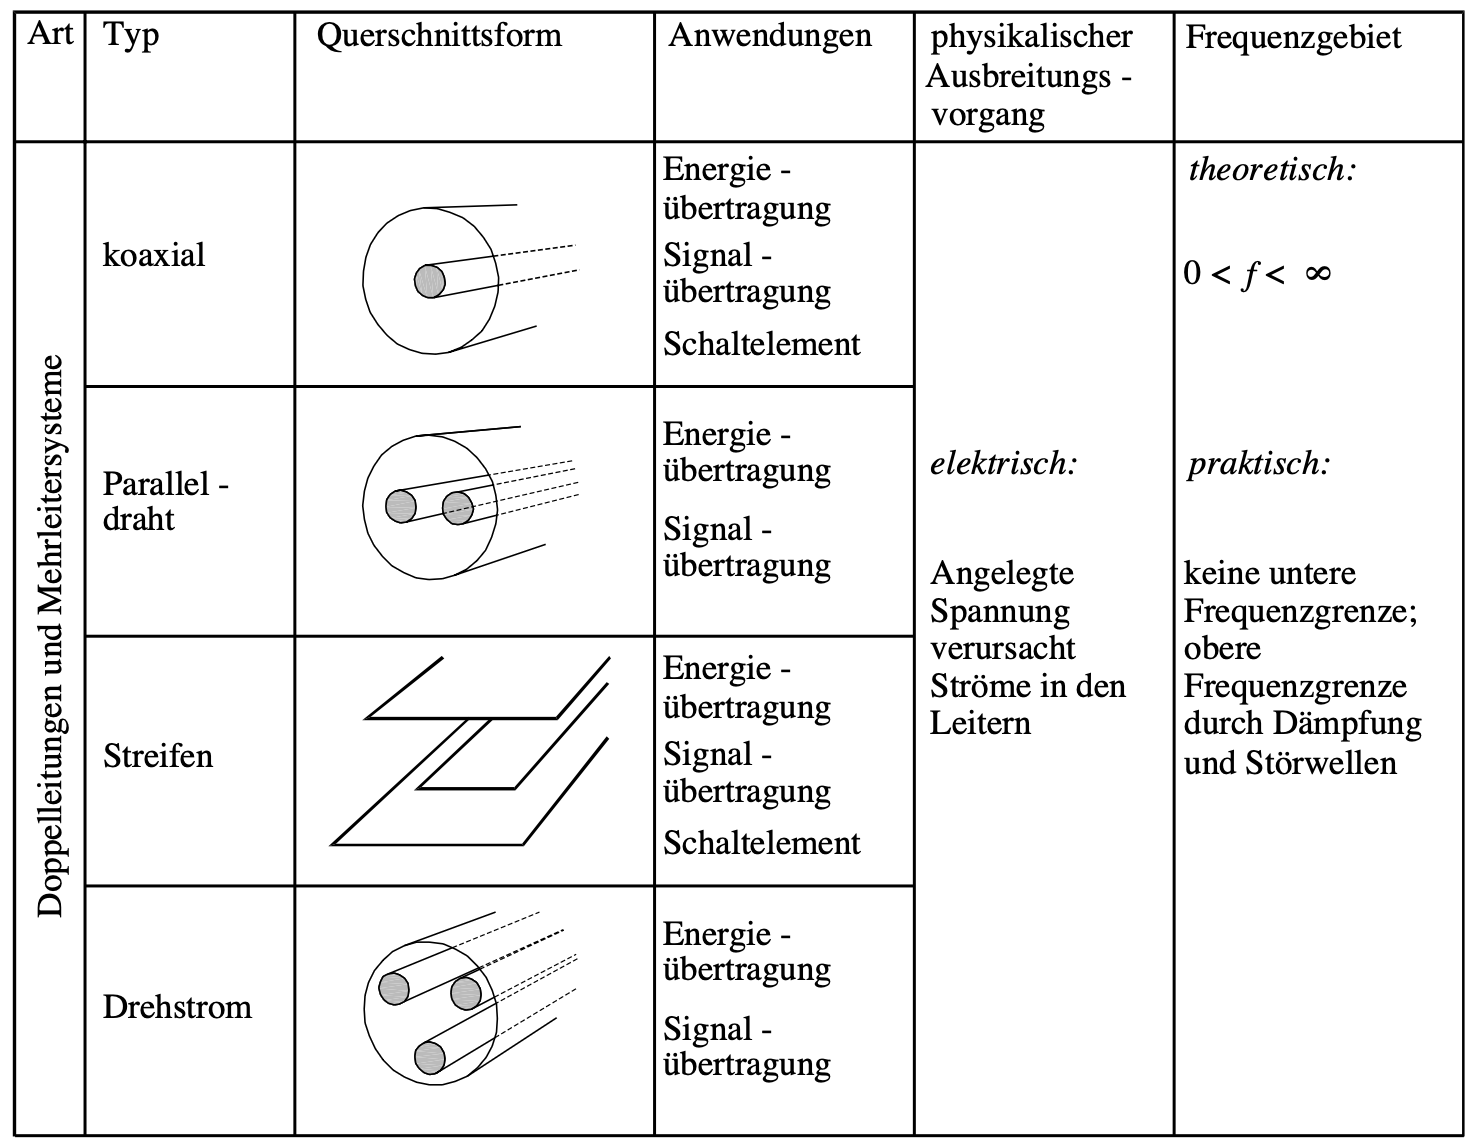
\includegraphics[width=0.75\textwidth]{../Ausarbeitung/images/Leiter.png}
    \end{center}
\end{figure}

\end{frame}


\begin{frame}{Leitungsbeläge}
Auf einem Leitungsstück der Länge $s$ mit Widerstand $R_{s}$ sehen elektrische und magnetische Felder
\begin{itemize}
    \item<1-> Induktion $L_{s}$
    \item<2-> Kapazität $C_{s}$ und
    \item<3-> Querleitwert $G_{s}$
\end{itemize}
\begin{figure}[!htb]
    \begin{center}
        \includegraphics[width=0.5\textwidth]{graphics/Ersatzschaltbild1/document}
    \end{center}
\end{figure}
\end{frame}


\begin{frame}{Leitungsbeläge}
Definiere Induktionsbelag $L^{\prime} = \frac{L_{s}}{s}$ als Längsinduktivität pro Längeneinheit.
Analog definieren wir
\begin{itemize}
    \item Kapazitätbelag $C^{\prime} = \frac{C_{s}}{s}$
    \item Leitwertsbelag $G^{\prime} = \frac{G_{s}}{s}$
    \item Widerstandsbelag $R^{\prime} = \frac{R_{s}}{s}$
\end{itemize}

\end{frame}


\begin{frame}{Ersatzschaltbild eines infinitesimalem Leitungsstücks}
Wir stellen uns ein infinitesimales Leitungsstück der Länge $\mathrm{d}z$ vor:
\begin{figure}[!htb]
    \begin{center}
        \includegraphics[width=0.5\textwidth]{graphics/Ersatzschaltbild2/document}
    \end{center}
\end{figure}
Am Ende des Leiterstücks liegen Spannung
\[
u(z + \mathrm{d}z) \approx u(z) + \frac{\partial u}{\partial z}(z) \, \mathrm{d}z
\] und Strom
\[
i(z + \mathrm{d}z) \approx i(z) + \frac{\partial i}{\partial z}(z) \, \mathrm{d}z
\] an.
\end{frame}


\begin{frame}{Spannung auf infinitesimalem Leitungsstück}
Entlang des Leitungsstücks verursachen Widerstand $R^{\prime} \, \mathrm{d}z$ und Induktivität
$L^{\prime} \, \mathrm{d}z$ einen Spannungsabfall von
\[
i(z, t) \, R^{\prime} \, \mathrm{d}z
+
\frac{\partial i(z, t)}{\partial t} \, L^{\prime} \, \mathrm{d}z.
\]
Mit der Kirchhoffschen Maschengleichung~\cite{Kirchhoff} folgt
\begin{equation*}
    u(z, t) = i(z, t) \, R^{\prime} \, \mathrm{d}z
    +
    \frac{\partial i(z, t)}{\partial t} \, L^{\prime} \, \mathrm{d}z
    + u(z + \mathrm{d}z, t).
\end{equation*}

\end{frame}


\begin{frame}{Strom auf infinitesimalem Leitungsstück}
Durch Querleitwert $G^{\prime} \, \mathrm{d}z$ und Querkapazität $C^{\prime} \, \mathrm{d}z$ fließt der Strom
\[
u(z + \mathrm{d}z, t) \, G^{\prime} \, \mathrm{d}z
+
\frac{\partial u(z + \mathrm{d}z, t)}{\partial t} \, C^{\prime} \, \mathrm{d}z.
\]
Mit der Kirchhoffschen Knotenregel~\cite{Kirchhoff} folgt
\begin{equation*}
    i(z, t) = u(z + \mathrm{d}z, t) \, G^{\prime} \, \mathrm{d}z
    +
    \frac{\partial u(z + \mathrm{d}z, t)}{\partial t} \, C^{\prime} \, \mathrm{d}z
    + i(z + \mathrm{d}z, t).
\end{equation*}

\end{frame}


\begin{frame}{Differentialgleichungen der elektrischen Leitung}
Durch Teilen beider Gleichungen durch $\mathrm{d}z$ erhalten wir die \alert{Gleichungen des elektrischen Leiters}
\begin{align}
    \frac{\partial u}{\partial z} &= -\left(R^{\prime} + L^{\prime}\frac{\partial}{\partial t}\right)i \label{eq:Dgl1}
    \\[1ex]
    \frac{\partial i}{\partial z} &= -\left(G^{\prime} + C^{\prime}\frac{\partial}{\partial t}\right)u. \label{eq:Dgl2}
\end{align}
Hieraus lassen sich die folgenden \alert{Telegraphenleitungen} herleiten:
\begin{align}
    \frac{\partial^{2} u}{\partial z^{2}} &= R^{\prime} G^{\prime} u(z,t) + (R^{\prime} C^{\prime} + L^{\prime}
    G^{\prime}) \frac{\partial u(z, t)}{\partial t} + L^{\prime} C^{\prime} \frac{\partial^{2} u(z,t)}{\partial t^{2}}
    \label{eq:Tele1} \\[1.5ex]
    \frac{\partial^{2} i}{\partial z^{2}} &= R^{\prime} G^{\prime} i(z,t) + (R^{\prime} C^{\prime} + L^{\prime}
    G^{\prime}) \frac{\partial i(z, t)}{\partial t} + L^{\prime} C^{\prime} \frac{\partial^{2} i(z, t)}{\partial t^{2}}.
\end{align}

\end{frame}


\section{Lösung der Gleichungen des elektrischen Leiters}


\begin{frame}{Eingeschwungener Zustand}
Wir machen folgende Annahmen:
\begin{itemize}
    \item<1-> ignoriere Einschwungvorgang
    \item<2-> zeitlich sinusförmiger Verlauf
    \item<3-> nur eine Schwingung mit Kreisfrequenz $\omega$
\end{itemize}

\vspace*{1em}
\onslide<4->{
Dann lassen sich Strom $i$ und Spannung $u$ mittels sogenannter Phasoren $\underline{I}$ und $\underline{U}$ darstellen:
\begin{align}
    u(z, t) &= \mathrm{Re} \left[ \underline{U}(z) \exp(\mathrm{j} \omega t) \right] \label{eq:Spannung} \\
    i(z, t) &= \mathrm{Re} \left[ \underline{I}(z) \exp(\mathrm{j} \omega t) \right]
\end{align}
}

\end{frame}


\begin{frame}{Differentialgleichungssystem}
Wir erhalten Wellengleichungen für $\underline{U}$ und $\underline{I}$:
\begin{align}
    \frac{\text{d}^{2} \underline{U}}{\text{d} z^{2}} &= \gamma^{2} \underline{U} \label{eq:VerlustDgl1} \\[1ex]
    \frac{\text{d}^{2} \underline{I}}{\text{d} z^{2}} &= \gamma^{2} \underline{I} \label{eq:VerlustDgl2} \\[1ex]
    \gamma^{2} &= \left( R^{\prime} + \mathrm{j} \omega L^{\prime} \right) \left( G^{\prime} + \mathrm{j} \omega
    C^{\prime} \right) \label{eq:Gamma}.
\end{align}
Man nennt $\gamma = \alpha + \mathbf{j} \beta$ die Wellenausbreitungskonstante.

\end{frame}


\begin{frame}{Allgemeine Lösung}
    Lösungen haben die Form
    \begin{equation}
        \underline{U}(z) = \underline{U}_{h_{0}} \mathbf{e}^{- \gamma z}
        +
        \underline{U}_{r_{0}} \mathbf{e}^{\gamma z}
        = \underline{U}_{h}(z) + \underline{U}_{r}(z) \label{eq:VerlustU}
    \end{equation}
    und
    \begin{equation}
        \underline{I}(z) = \frac{1}{Z_{w}} \left( \vphantom{\sqrt{1}{Z}}
        \underline{U}_{h_{0}} \mathbf{e}^{- \gamma z} - \underline{U}_{r_{0}} \mathbf{e}^{\gamma z} \right)
        = \underline{I}_{h}(z) + \underline{I}_{r}(z), \label{eq:VerlustI}
    \end{equation}
    wobei
    \begin{equation}
        Z_{w} = \sqrt{\frac{R^{\prime} + \mathrm{j} \omega L^{\prime}}{G^{\prime} + \mathrm{j} \omega C^{\prime}}}
        \label{eq:Zw}
    \end{equation}
    Wellenwiderstand genannt wird.


    Wir bezeichnen mit $\underline{U}_{h}$ die \alert{hinlaufende}, mit $\underline{U}_{r}$ die
    \alert{rücklaufende} Welle. Für $\underline{I}_{h}$ und $\underline{I}_{r}$ gilt analoges.

\end{frame}


\begin{frame}{Verlustlose Leitung}
Der verlustlose Fall ist gegeben durch \mbox{$R^{\prime} = G^{\prime} = 0$}.
Es folgt
\[
Z_{w} = \sqrt{\frac{L^{\prime}}{C^{\prime}}}
\]
und da $\alpha = 0$ gilt
\[
\gamma = \mathbf{j} \beta = \mathbf{j} \omega \sqrt{L^{\prime} C^{\prime}}.
\]
Somit ist der Wellenwiderstand \alert{reell}, die Wellenausbreitungskonstante hingegen
\alert{imaginär}.
\end{frame}


\begin{frame}{Wellenlänge}
Die Spannungen im Abstand einer Wellenlänge $\lambda$ erfüllen
\begin{equation}
\underline{U}(\lambda) =
\underline{U}_{h_{0}} \mathbf{e}^{- \mathrm{j} \beta \lambda}
+
\underline{U}_{r_{0}} \mathbf{e}^{\mathrm{j} \beta \lambda}
= \underline{U}_{h_{0}} + \underline{U}_{r_{0}}
= \underline{U}(0)
\end{equation}
und somit
\[
\mathbf{e}^{- \mathrm{j} \beta \lambda} = \mathbf{e}^{\mathrm{j} \beta \lambda} = 1.
\]
Es folgt
\[
\lambda = \frac{2 \pi}{\beta}.
\]
\end{frame}


\begin{frame}{Impedanz vs. Wellenwiderstand}
Für die Impedanz gilt
\begin{equation*}
    Z(z) = \frac{\underline{U}(z)}{\underline{I}(z)} =
     \frac{\underline{U}_{h}(z) + \underline{U}_{r}(z)}{\underline{I}_{h}(z) +
     \underline{I}_{r}(z)} \ne const.
\end{equation*}
entlang des Leiters, aber
\[ \frac{\underline{U}_{h}(z)}{\underline{I}_{h}(z)}
= \frac{\underline{U}_{r}(z)}{- \underline{I}_{r}(z)} = Z_{w}! \]

\end{frame}


\begin{frame}{Prinzip der Wellenausbreitung entlang eines Leiters}

    \begin{figure}[!htb]
        \begin{center}
            \documentclass{standalone}
\usepackage{tikz}
\usepackage{pgfplots}
\pgfplotsset{compat=1.18}
\usetikzlibrary{calc}
\usetikzlibrary{arrows.meta}

\begin{document}
\begin{tikzpicture}
\begin{axis}[
scale only axis,
xmin=0, xmax=25, ymin=-1, ymax=1,
axis x line=center,
axis y line=left,
axis lines=middle, % Place axes in the middle
xlabel={$z$}, % Label for x-axis
%      xlabel style={at={(axis description cs:1,0.45)}},
ylabel={}, % Label for y-axis
samples=150, % Number of samples for smooth curve
yticklabels={},
ytick=\empty,
xtick={25},
xticklabels={$l$},
enlargelimits=0.11, % Ensure axes extend slightly beyond data
y axis line style={-}, % No arrows on y axis
x axis line style={->}, % Arrow on axes
separate axis lines,
]

% manually place 0 tickmark
\node[below=3pt, xshift=5pt] at (axis cs:0,0) {0};

% hinlaufende Welle
\addplot[dashed, thick, domain=0:25] {exp(-0.03*x)} node [pos=0.5, above, inner sep=5pt] {$\mathrm{e}^{- \alpha z}$}
node[inner sep=2pt, right] (P1) {};
\addplot[dashed, thick, domain=0:25] {-exp(-0.03*x)} node[inner sep=2pt, right] (P2) {};
\addplot[blue, thick, domain=0:25] {exp(-0.03*x)*cos(deg(x))} node[pos=0.03, inner sep=0] (H1) {} node[pos=0.04, inner
sep=0] (H2) {};
\draw (H1) -- +(35:0.5cm) node[right, inner sep=2pt] {$u_{h}$};
\draw[-Stealth] (H2) -- +(0:0.5cm);

% ruecklaufende Welle
\addplot[dashed, thick, domain=6:25] {0.25*exp(-0.05*(25-x))} node [pos=0.5, above, inner sep=4pt, xshift=-1pt]
{$\mathrm{e}^{-
\alpha (l-z)}$};
\addplot[dashed, thick, domain=6:25] {-0.25*exp(-0.05*(25-x))};
\addplot[blue, thick, densely dotted, domain=6:25] {0.25*exp(-0.05*(25-x))*cos(deg(x))} node[pos=0.97, inner sep=0]
(R1) {} node[pos=0.62, inner sep=0] (R2) {};
\draw (R1) -- +(25:0.5cm) node[right, inner sep=2pt] {$u_{r}$};
\draw[-Stealth] (R2) -- +(0:-0.5cm);

\draw (P1) -- (P2);

\end{axis}

\end{tikzpicture}

\end{document}
        \end{center}
    \end{figure}

\end{frame}


\begin{frame}{Wellenausbreitung für den verlustlosen Fall}
Die schwarzen Hüllkurven sind jeweils durch
\[
\mathrm{Re} ( \left| \underline{U}_{h}(z) + \underline{U}_{r}(z) \right| )
\quad \text{bzw.}
- \mathrm{Re} ( \left| \underline{U}_{h}(z) + \underline{U}_{r}(z) \right| )
\] gegeben. Die Maxima der Amplituden laufen auf der oberen, die Minima auf der unteren Hüllkurve
für alle $t$.
\begin{figure}[H]
    \begin{minipage}{0.32\textwidth}
        \centering
        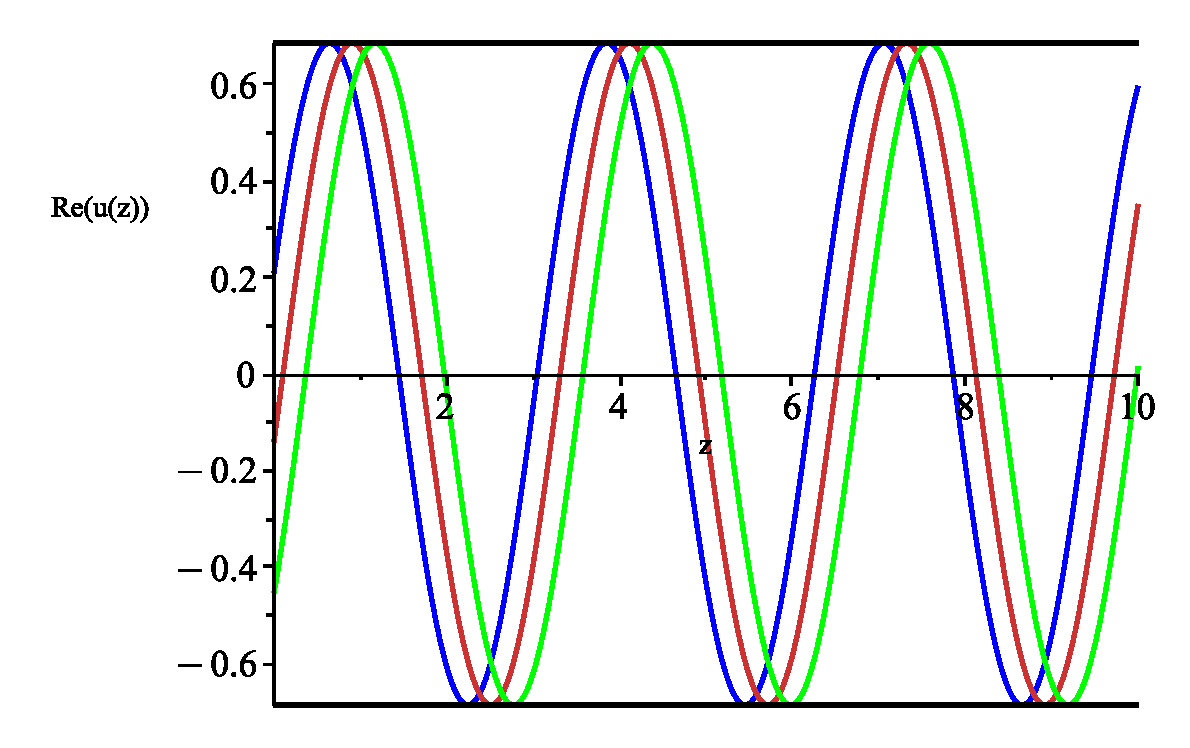
\includegraphics[width=\linewidth]{../graphics/Enveloppe/verlustlos/R0}
        \caption*{$r=0$, $t=0.1$ (blau), $t=0.2$ (orange) und $t=0.3$ (grün)}
    \end{minipage}
    \hfill
    \begin{minipage}{0.32\textwidth}
        \centering
        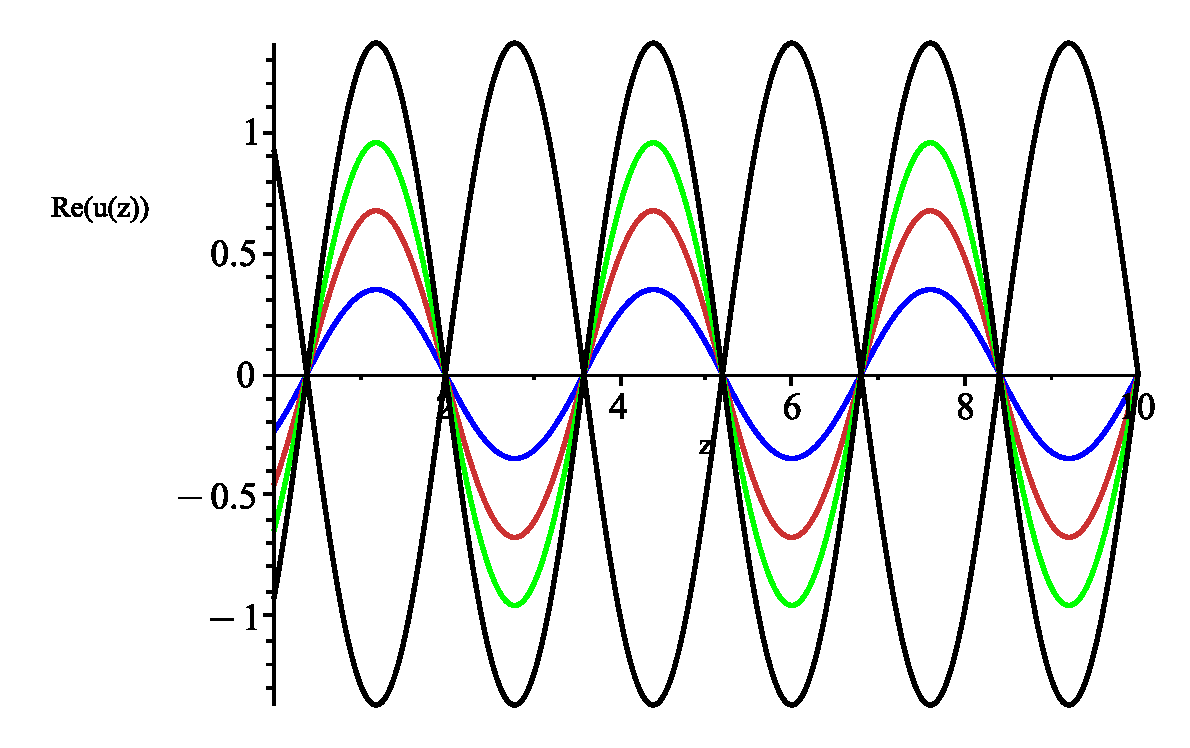
\includegraphics[width=\linewidth]{../graphics/Enveloppe/verlustlos/R-1}
        \caption*{$r=-1$, $t=0.05$ (blau), $t=0.1$ (orange) und $t=0.15$ (grün)}
    \end{minipage}
    \hfill
    \begin{minipage}{0.32\textwidth}
        \centering
        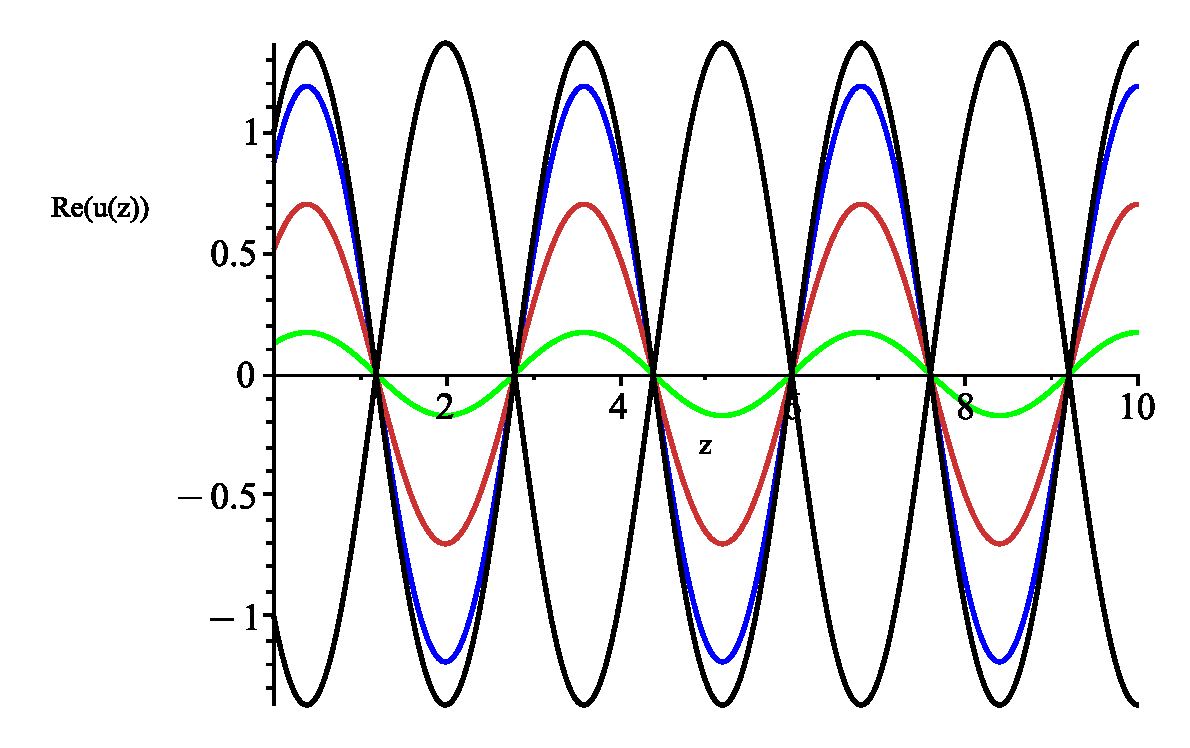
\includegraphics[width=\linewidth]{../graphics/Enveloppe/verlustlos/R1}
        \caption*{$r=1$, $t=0.1$ (blau), $t=0.2$ (orange) und $t=0.28$ (grün)}
    \end{minipage}
\end{figure}
\end{frame}


\begin{frame}{Wellenausbreitung für den verlustbehafteten Fall}
    \begin{figure}[H]
    \begin{minipage}{0.32\textwidth}
        \centering
        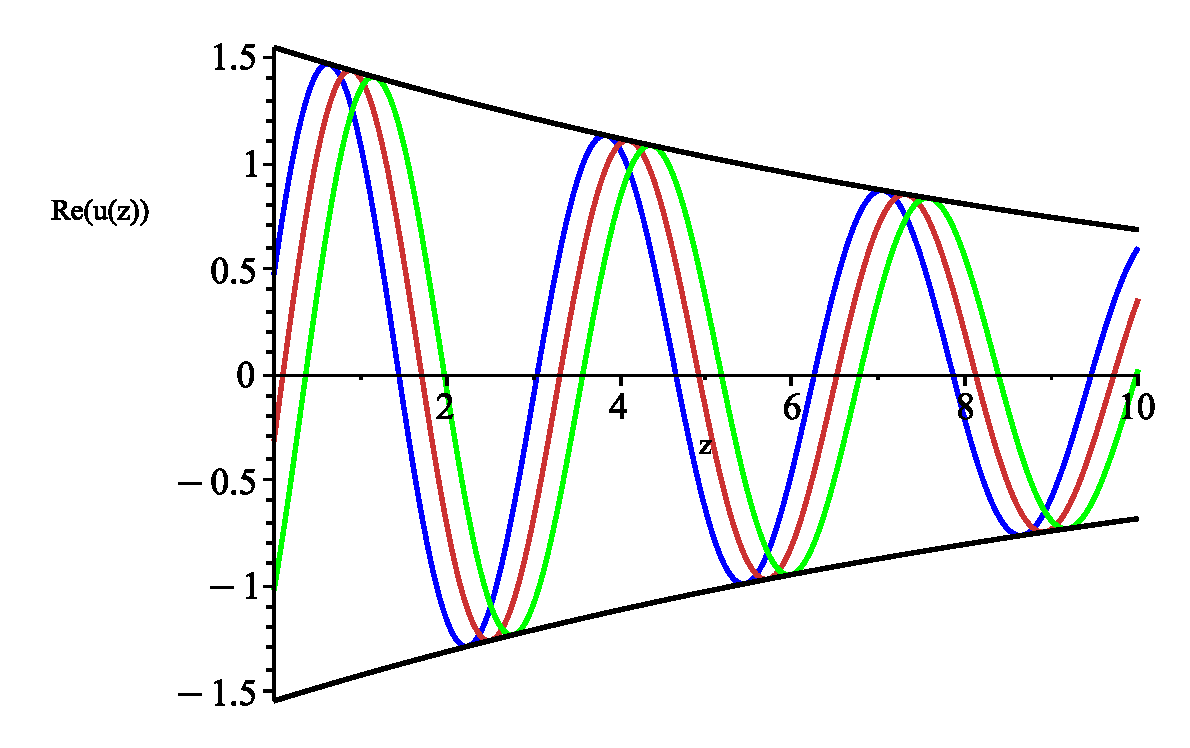
\includegraphics[width=\linewidth]{../graphics/Enveloppe/verlustbehaftet/R0}
        \caption*{$r=0$, $t=0.1$ (blau), $t=0.2$ (orange) und $t=0.3$ (grün)}
    \end{minipage}
    \hfill
    \begin{minipage}{0.32\textwidth}
        \centering
        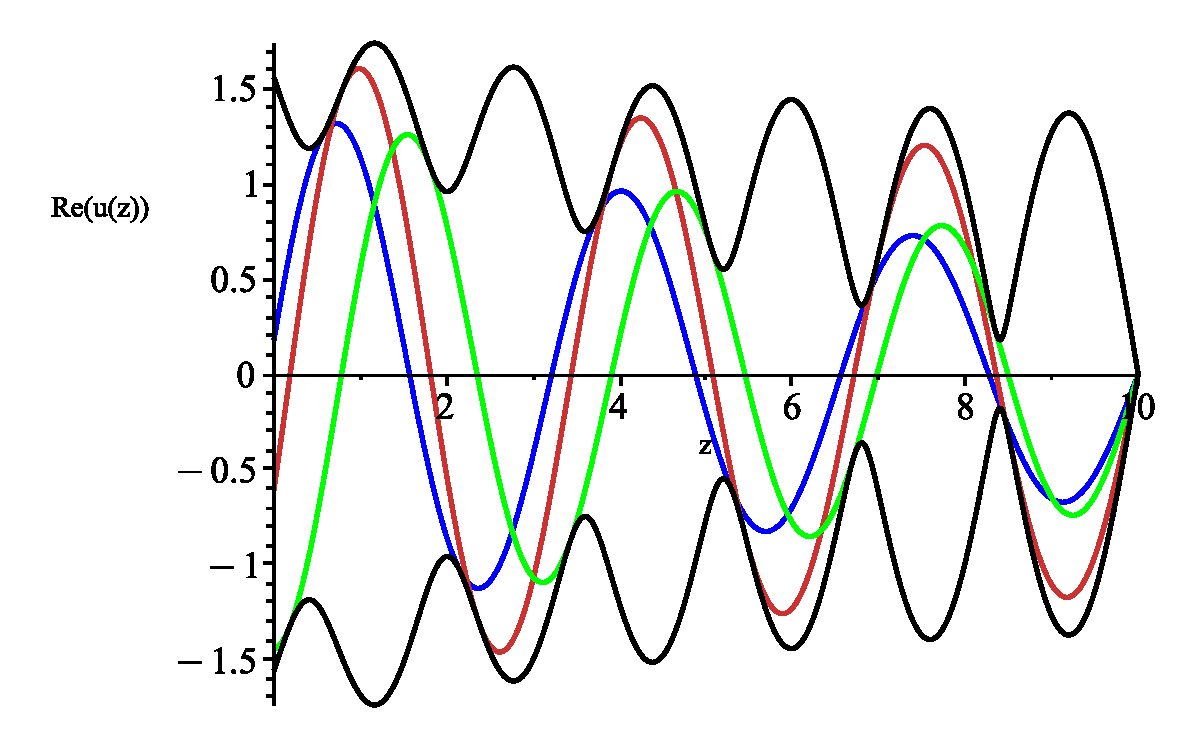
\includegraphics[width=\linewidth]{../graphics/Enveloppe/verlustbehaftet/R-1}
        \caption*{$r=-1$, $t=0.1$ (blau), $t=0.2$ (orange) und $t=0.5$ (grün)}
    \end{minipage}
    \hfill
    \begin{minipage}{0.32\textwidth}
        \centering
        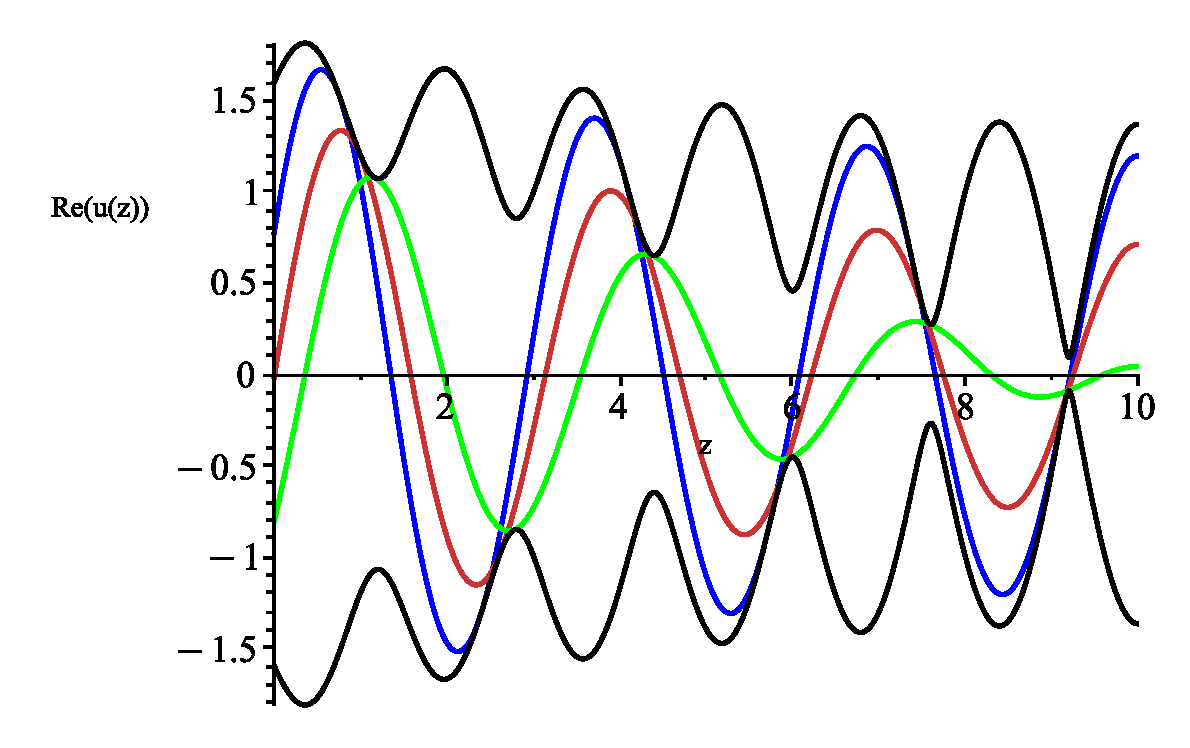
\includegraphics[width=\linewidth]{../graphics/Enveloppe/verlustbehaftet/R1}
        \caption*{$r=1$, $t=0.1$ (blau), $t=0.2$ (orange) und $t=0.3$ (grün)}
    \end{minipage}
\end{figure}
\end{frame}


\begin{frame}{Randbedingungen am Leiteranfang}
Bei den Wellengleichungen \eqref{eq:VerlustDgl1} und \eqref{eq:VerlustDgl2} handelt es sich um
gewöhnliche Differentialgleichungen 2.~Ordnung. Wir müssen daher jeweils zwei Randbedingungen für
eine eindeutige Lösung festlegen.

\vspace{1ex}
Sei
\begin{align*}
    \underline{U}(0) &= \underline{U}_{a} = \underline{U}_{h_{0}} + \underline{U}_{r_{0}} \\[1ex]
    \underline{I}(0) &= \underline{I}_{a} = \frac{1}{Z_{w}}
    \left(
    \vphantom{\sqrt{1}{Z_{w}}}
    \underline{U}_{h_{0}} - \underline{U}_{r_{0}} \right).
\end{align*}
Es folgt für die Integrationskonstanten $\underline{U}_{h_{0}}$ und $\underline{U}_{r_{0}}$
\[ \underline{U}_{h_{0}} = \frac{\underline{U}_{a} + Z_{w} \underline{I}_{a}}{2}
\quad \text{und} \quad
\underline{U}_{h_{0}} = \frac{\underline{U}_{a} - Z_{w} \underline{I}_{a}}{2}. \]
\end{frame}


\begin{frame}{Randbedingungen am Leiteranfang}
Damit lauten die Gleichungen für Spannung und Strom entlang der Leitung
\begin{align}
    \underline{U}(z) &=
    \frac{1}{2} \left( \underline{U}_{a} + Z_{w} \underline{I}_{a} \right) \mathbf{e}^{- \gamma z}
    +
    \frac{1}{2} \left( \underline{U}_{a} - Z_{w} \underline{I}_{a} \right) \mathbf{e}^{\gamma z} \label{eq:UxA}
    \\[1ex]
    \underline{I}(z) &=
    \frac{1}{2} \left( \frac{\underline{U}_{a}}{Z_{w}} + \underline{I}_{a} \right) \mathbf{e}^{- \gamma z}
    -
    \frac{1}{2} \left( \frac{\underline{U}_{a}}{Z_{w}} - \underline{I}_{a} \right) \mathbf{e}^{\gamma z}
    \label{eq:IxA}
    .
\end{align}
\end{frame}


\begin{frame}{Randbedingungen am Leiterende}
Für $z=l$ sei
\begin{align*}
    \underline{U}(l) &= \underline{U}_{e} = \underline{U}_{h_{0}} \mathbf{e}^{- \gamma l}
    +
    \underline{U}_{r_{0}} \mathbf{e}^{ \gamma l} \\[1ex]
    \underline{I}(l) &= \underline{I}_{e} = \frac{1}{Z_{w}}
    \left(
    \underline{U}_{h_{0}} \mathbf{e}^{- \gamma l}
    -
    \underline{U}_{r_{0}} \mathbf{e}^{ \gamma l}
    \right).
\end{align*}
In diesem Fall gilt für die Integrationskonstanten
\[ \underline{U}_{h_{0}} = \frac{\underline{U}_{e} + Z_{w} \underline{I}_{e}}{2} \mathbf{e}^{\gamma l}
\quad \text{und} \quad
\underline{U}_{r_{0}} = \frac{\underline{U}_{e} - Z_{w} \underline{I}_{e}}{2} \mathbf{e}^{- \gamma l}. \]
Die Gleichungen für Spannung und Strom lauten damit
\begin{align}
    \underline{U}(z) &=
    \frac{1}{2} \left( \underline{U}_{e} + Z_{w} \underline{I}_{e} \right) \mathbf{e}^{\gamma (l - z)}
    +
    \frac{1}{2} \left( \underline{U}_{e} - Z_{w} \underline{I}_{e} \right) \mathbf{e}^{- \gamma (l - z)} \label{eq:UxE}
    \\[1ex]
    \underline{I}(z) &=
    \frac{1}{2} \left( \frac{\underline{U}_{e}}{Z_{w}} + \underline{I}_{e} \right) \mathbf{e}^{\gamma (l - z)}
    -
    \frac{1}{2} \left( \frac{\underline{U}_{e}}{Z_{w}} - \underline{I}_{e} \right) \mathbf{e}^{- \gamma (l - z)}
    \label{eq:IxE} .
\end{align}

\end{frame}


\section{Reflexionsfaktor}


\begin{frame}{Reflexionsfaktor}
\begin{figure}[!htb]
    \begin{center}
        \documentclass{standalone}

\usepackage{tikz}
\usepackage[europeanresistors]{circuitikz}
\usetikzlibrary{decorations.markings}
\usetikzlibrary{arrows.meta}
\usetikzlibrary{calc}

\begin{document}

\begin{circuitikz}

\tikzset{
    fieldline/.style={postaction={decorate}, decoration={markings}},
    arrow/.style={decoration={mark=at position #1 with {\arrow{Stealth}}}},
    reversearrow/.style={decoration={mark=at position #1 with {\arrowreversed{Stealth}}}},
    line style/.style={solid, black}
    resistor label/.style={l=$R_{x}$}}

\coordinate (A1) at (1, 10);
\coordinate (A2) at (3, 10);
\coordinate (A3) at (7, 10);
\coordinate (A4) at (1, 9);
\coordinate (A5) at (1, 7);
\coordinate (A6) at (1, 5);
\coordinate (A7) at (3, 5);
\coordinate (A8) at (7, 5);
\coordinate (A9) at (9, 10);
\coordinate (A10) at (9, 9);
\coordinate (A11) at (9, 6);
\coordinate (A12) at (9, 5);

\draw (A1) -- ($(A2) + (2pt, 0)$) node[above] {$\underline{U}_{a} = Z_{w} \underline{I}_{a}$};
\draw (A1) -- (A4);

% Lastwiderstand
\draw (A4) to[european resistor, l=$Z_{0}$] (A5);

% voltage source
\draw (A5) to[sinusoidal voltage source, l=$U_{0}$] (A6);

\draw (A6) -- ($(A7) + (2pt, 0)$);

\draw[-Stealth, shorten >=5pt, shorten <=5pt] (A2) -- (A7) node[pos=0.5, right] {$\underline{U}_{a}$};

\draw[{Circle[open, fill=white]}-] ($(A2) + (-2pt, 0)$) -- ($(A2)!0.3!(A3)$);
\draw[dotted] ($(A2)!0.3!(A3)$) -- ($(A2)!0.7!(A3)$);
\draw[-{Circle[open, fill=white]}] ($(A2)!0.7!(A3)$) -- (A3);

\draw[{Circle[open, fill=white]}-] ($(A7) + (-2pt, 0)$) -- ($(A7)!0.3!(A8)$);
\draw[dotted] ($(A7)!0.3!(A8)$) -- ($(A7)!0.7!(A8)$);
\draw[-{Circle[open, fill=white]}] ($(A7)!0.7!(A8)$) -- (A8);

\draw[-Stealth, shorten >=5pt, shorten <=5pt] ($(A3) + (-2pt, 0)$) -- ($(A8) + (-2pt, 0)$) node[pos=0.5, left]
{$\underline{U}_{e}$};

\draw (A3) -- (A9) -- (A10);

% Wellenwiderstand
\draw (A10) to[european resistor, l=$Z_{w}$] (A11);

\draw (A11) -- (A12) -- (A8);

\end{circuitikz}

\end{document}
    \end{center}
\end{figure}

Das Verhältnis beider Teilspannungen entlang der Leitung ist
\[
r(z) = \frac{\underline{U}_{r}(z)}{\underline{U}_{h}(z)} =
       \frac{Z_{e}-Z_{w}}{Z_{e}+Z_{w}} \mathbf{e}^{-2 \gamma (l-z)}.
\]
$r$ wird Reflexionsfaktor genannt. Am Leiterende gilt
\begin{equation}
    r(l)
    = \frac{\underline{U}_{r}(l)}{\underline{U}_{h}(l)}
    = \frac{- \underline{I}_{r}(l)}{\underline{I}_{h}(l)}
    = \frac{Z_{e}-Z_{w}}{Z_{e}+Z_{w}} \label{eq:RFactor}.
\end{equation}

\end{frame}


\begin{frame}{Transformation der Impedanz}
Setzen wir
\[
\frac{\underline{U}(z)}{\underline{I}(z)}
= \frac{\underline{U}_{h}(z) +
\underline{U}_{r}(z)}{\underline{I}_{h}(z) +
    \underline{I}_{r}(z)} = Z(z),
\]
so folgt mit~\eqref{eq:RFactor}
\[
Z(z) = \frac{1 + r(z)}{1 - r(z)} Z_{w}.
\]
\end{frame}


\begin{frame}{Anpassung}
Im Falle der Anpassung gilt $Z_{e} = Z_{w}$.
\begin{itemize}
    \item <1-> $r = 0$, d.\,h. es findet keine Reflexion statt
    \item <2-> es folgt $\underline{U}_{r}(z) = 0$ (für \alert{alle} $z$!)
    \item <3-> einlaufende Welle wird am Leitungsende vollkommen absorbiert!
    \item <4-> wichtiger Fall in der Praxis da keine unerwünschten Interferenzen auftreten
    \item <5-> das Signal wird ungestört übertragen
\end{itemize}
\end{frame}


\begin{frame}{Kurzschluss am Leitungsende}
Gilt am Leiterende $Z_{e} = 0$, so folgt $r = -1$ und somit
\[
\underline{U}_{r}(l) = - \underline{U}_{h}(l).
\]

\begin{itemize}
    \item<2-> aus \eqref{eq:IxE} folgt $\underline{U}(l) = \underline{U}_{e} = 0$
    \item<3-> hinlaufende Welle wird am Leitungsende vollkommen reflektiert
    \item<4-> hin- und rücklaufende Welle sind am Leiterende um $\pi$ phasenverschoben
\end{itemize}

\end{frame}


\begin{frame}{Offene Leitung}
Eine offene Leitung ist durch $Z_{e} \gg 1$ gekennzeichnet. Es folgt $r = 1$ und somit
\[
\underline{I}_{r}(l) = - \underline{I}_{h}(l).
\]

\begin{itemize}
    \item<2-> aus \eqref{eq:IxE} folgt $\underline{I}(l) = \underline{I}_{e} = 0$
    \item<3-> hinlaufende Welle wird am Leitungsende ebenfalls vollkommen reflektiert
    \item<4-> hin- und rücklaufende Welle sind am Leiterende in Phase
\end{itemize}

\end{frame}


\begin{frame}{Kurzschluss/Offene Leitung im verlustlosen Fall}
Im verlustloses Fall betrachten wir nochmals
\[
r(z) = \frac{\underline{U}_{r}(z)}{\underline{U}_{h}(z)} =
\frac{Z_{e}-Z_{w}}{Z_{e}+Z_{w}} \, \mathbf{e}^{-\mathbf{j} 2 \beta (l-z)}.
\]
$r$ ändert seine Phase, nicht aber seinen Betrag.
\vspace{1ex}

Für den Kurzschluss ist $r=-1$. Wegen $|r|=1$ wird somit ein Kurzschluss in einen Leerlauf und
umgekehrt transformiert!

\vspace{1ex}
Dies passiert im Abstand $\nicefrac{\lambda}{4}$, denn es gilt mit $l - z = \Delta z$
\[
\mathbf{e}^{- \mathbf{j} 2 \beta \frac{\lambda}{4}} =
\mathbf{e}^{- \mathbf{j} 2 \frac{2 \pi}{\lambda} \frac{\lambda}{4}} =
\mathbf{e}^{- \mathbf{j} \pi} = -1.
\]
\end{frame}


\begin{frame}{Kurzschluss/Offene Leitung im verlustlosen Fall}
Sei $r(l) = r_{0}$ mit $r_{0} = \pm 1$ und
$\varphi = - 2 \beta \Delta z = - \frac{4 \pi}{\lambda} \Delta z$.
Es folgt
\[
Z = \frac{1 + r}{1 - r} Z_{w} =
\frac{1 + r_{0} \mathbf{e}^{\mathbf{j} \varphi}}{1 - r_{0} \mathbf{e}^{\mathbf{j} \varphi}} Z_{w}.
\] Mit der Eulerschen Formel folgt
\[
Z = \mathbf{j} \frac{r_{0} \sin \varphi}{1 - r_{0} \cos \varphi} Z_{w}.
\]
Für $\varphi \ne n \pi$ bzw. $\Delta z \ne n \frac{\lambda}{4}$, $n \in - \mathbb{N}$, ist $Z$ eine
rein imaginäre Größe.

Ist insbesondere die Leiterlänge $l$ kein Vielfaches von $\nicefrac{\lambda}{4}$, dann ist die Impedanz am
Anfang des Leiters imaginär!
\end{frame}

\begin{frame}{Imaginäre Impedanzen}
\begin{figure}[H]
    \begin{minipage}{0.45\textwidth}
        \centering
        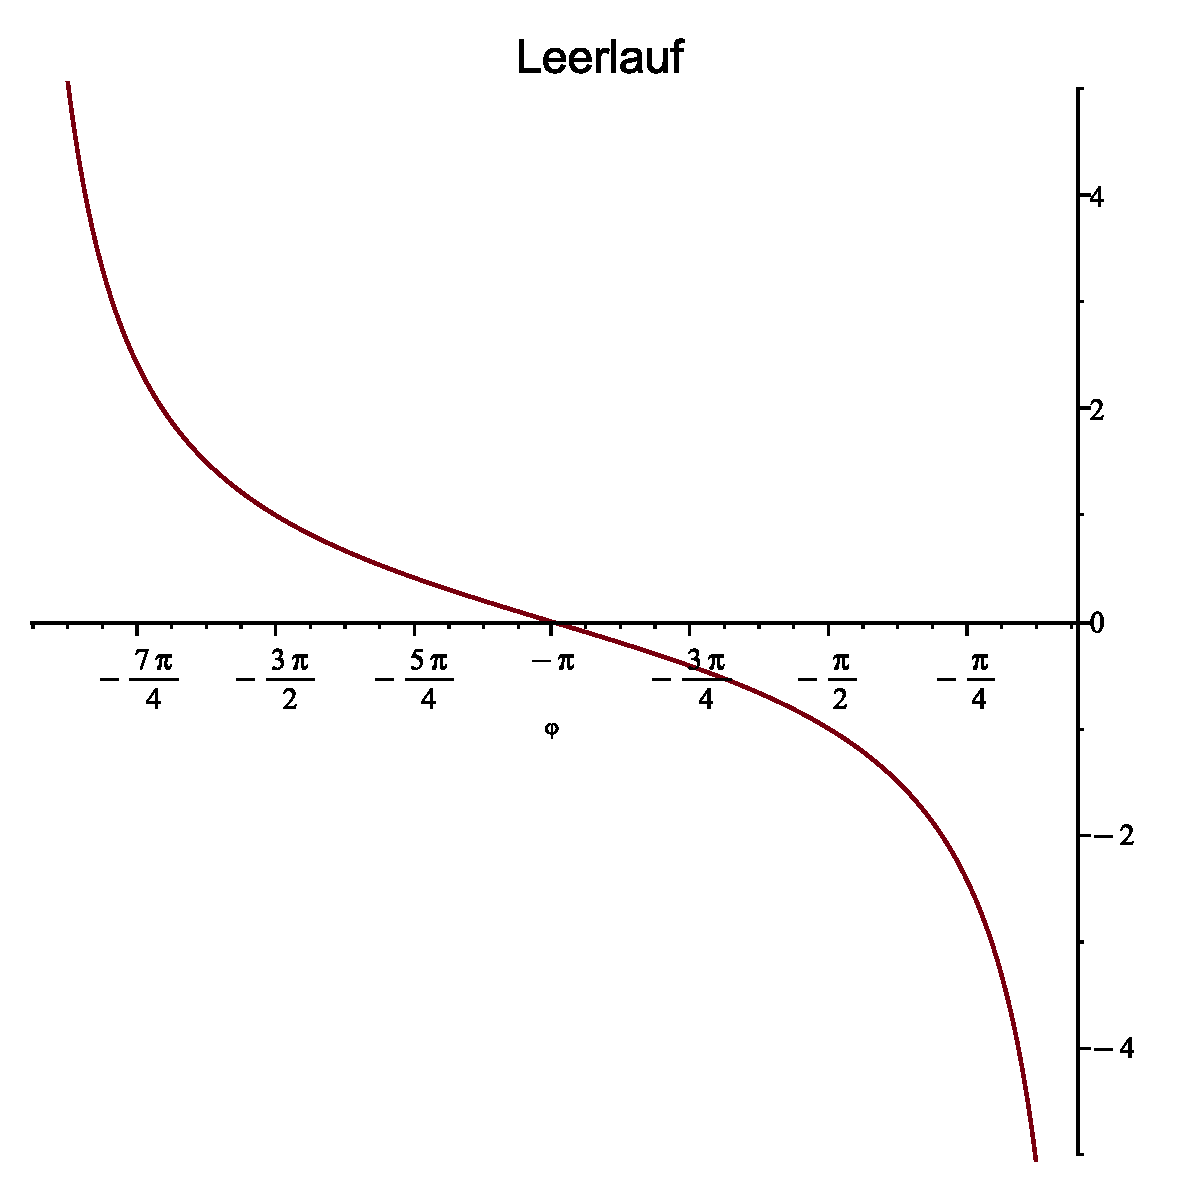
\includegraphics[width=\linewidth]{graphics/ImpedanzLeerlauf}
        \caption*{$r_{0}=1$}
    \end{minipage}
    \hfill
    \begin{minipage}{0.45\textwidth}
        \centering
        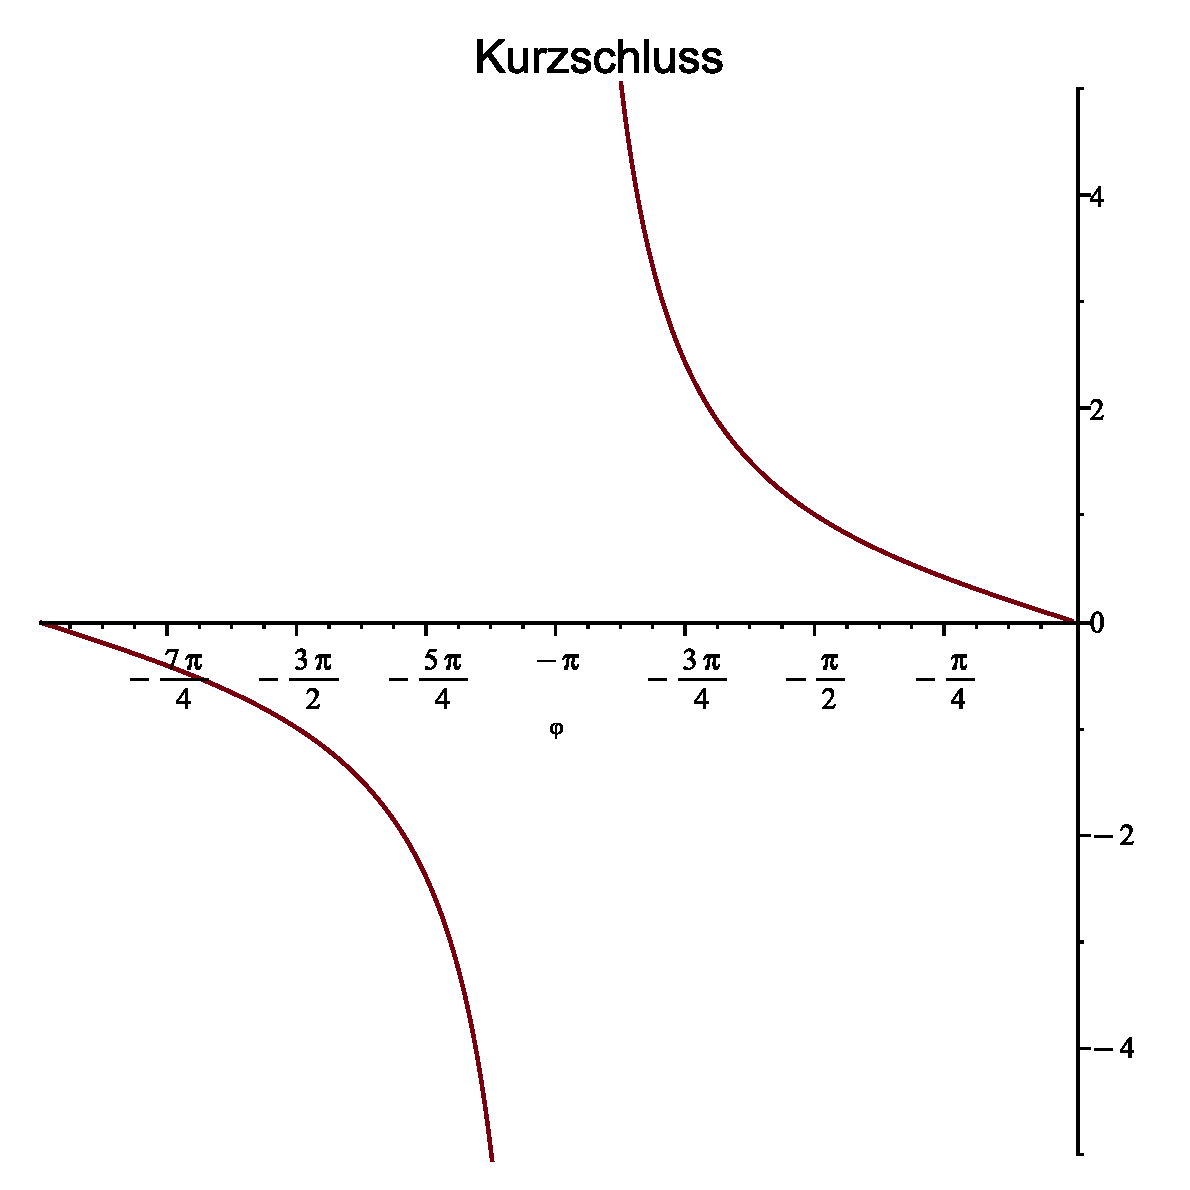
\includegraphics[width=\linewidth]{graphics/ImpedanzKurzschluss}
        \caption*{$r_{0}=-1$}
    \end{minipage}
\end{figure}
\end{frame}


\begin{frame}{Beliebige Kapazitäten und Induktivitäten}
Es folgt für
\begin{itemize}
    \item $0 < \Delta z < \frac{\lambda}{4} \Rightarrow \mathrm{Im}(Z) > 0$: die Leitung verhält
    sich wie eine Induktivität
    \item $\frac{\lambda}{4} < \Delta z < \frac{\lambda}{2} \Rightarrow \mathrm{Im}(Z) < 0$: die
    Leitung verhält sich wie eine Kapazität
\end{itemize}

Ein solcher Leiter speichert nahezu verlustfrei dies gesamte elektrische Energie
im elektrischen Feld (Kapazität) bzw. im magnetischen Feld (Induktivität).

\end{frame}


\begin{frame}{Literaturverzeichnis}
\printbibliography
\end{frame}

\end{document}
